\section{Examine the existence of limit cycle and periodic solution of the system:If periodic solutions exist, find them and sketch the phase portrait.}
$$\dot{x} = -y + x(1 - x^2 - y^2)$$$$\dot{y} = x + y(1 - x^2 - y^2)$$
\subsection*{Solution:}
Consider the non-linear autonomous dynamical system:
\begin{align*}
    \dot{x} &= -y + x(1 - x^2 - y^2)=P(x,y) \\
    \dot{y} &= x + y(1 - x^2 - y^2)=Q(x,y)
\end{align*}
now, $P(x, y) = -y + x(1 - x^2 - y^2)$ and $Q(x, y) = x + y(1 - x^2 - y^2)$.

\noindent Computing partial derivatives:
\[
\frac{\partial P}{\partial x} = (1 - x^2 - y^2) + x(-2x) = 1 - 3x^2 - y^2
\]
\[
\frac{\partial Q}{\partial y} = (1 - x^2 - y^2) + y(-2y) = 1 - x^2 - 3y^2
\]

\noindent Calculating the divergence of the vector field:
\[
\nabla \cdot \mathbf{f} = \frac{\partial P}{\partial x} + \frac{\partial Q}{\partial y} = 2 - 4x^2 - 4y^2 = 2 \left[ 1 - 2(x^2 + y^2) \right]
\]

\noindent Since $\frac{\partial P}{\partial x} + \frac{\partial Q}{\partial y}$ changes sign, Bendixson's negative criterion does not rule out the existence of closed trajectories.
Using the transformation $x = r \cos\theta$ and $y = r \sin\theta$, where $r^2 = x^2 + y^2$:
Differentiating $r^2 = x^2 + y^2$ with respect to $t$:
\[
2r\dot{r} = 2x\dot{x} + 2y\dot{y} \implies r\dot{r} = x\dot{x} + y\dot{y}
\]
Substituting $\dot{x}$ and $\dot{y}$:
\begin{align*}
    x\dot{x} + y\dot{y} &= x \left[ -y + x(1 - r^2) \right] + y \left[ x + y(1 - r^2) \right] \\
    &= -xy + x^2(1 - r^2) + xy + y^2(1 - r^2) \\
    &= (x^2 + y^2)(1 - r^2) = r^2(1 - r^2)
\end{align*}
Equating $r\dot{r} = r^2(1 - r^2)$ (for $r \neq 0$):
\[
\dot{r} = r(1 - r^2)
\]

\subsubsection*{ Angular Equation ($\dot{\theta}$)}
Using $r^2 \dot{\theta} = x\dot{y} - y\dot{x}$:
\begin{align*}
    x\dot{y} - y\dot{x} &= x \left[ x + y(1 - r^2) \right] - y \left[ -y + x(1 - r^2) \right] \\
    &= x^2 + xy(1 - r^2) + y^2 - xy(1 - r^2) \\
    &= x^2 + y^2 = r^2
\end{align*}
Equating $r^2 \dot{\theta} = r^2$:
\[
\dot{\theta} = 1
\]
\[
\frac{d\theta}{dt} = 1 \implies \theta(t) = t + \theta_0
\]
Setting phase angle $\theta_0 = 0$ for simplicity gives $\theta(t) = t$.

Separating variables in $\frac{dr}{dt} = r(1 - r^2)$:
\[
\frac{dr}{r(1 - r^2)} = dt
\]
Applying partial fraction decomposition:
\[
\int \left( \frac{1}{r} + \frac{r}{1 - r^2} \right) dr = \int dt
\]
\[
\ln r - \frac{1}{2}\ln|1 - r^2| = t + k
\]
\[
\ln \left( \frac{r}{\sqrt{|1 - r^2|}} \right) = t + k \implies \frac{r^2}{|1 - r^2|} = C_1 e^{2t} \quad (C_1 = e^{2k})
\]
Solving for $r^2$:
\[
r^2 = \frac{C_0 e^{2t}}{1 + C_0 e^{2t}} = \frac{1}{1 + C e^{-2t}} \quad \left( C = \frac{1}{C_0} \right)
\]
With initial condition $r(0) = r_0$, we obtain $C = \frac{1 - r_0^2}{r_0^2}$:
\[
r(t) = \frac{1}{\sqrt{1 + \left( \frac{1 - r_0^2}{r_0^2} \right) e^{-2t}}}
\]
\begin{align*}
    \therefore x(t) &= r(t)\cos(t) = \frac{\cos t}{\sqrt{1 + \left( \frac{1 - r_0^2}{r_0^2} \right) e^{-2t}}} \\[0.5em]
    \text{and} y(t) &= r(t)\sin(t) = \frac{\sin t}{\sqrt{1 + \left( \frac{1 - r_0^2}{r_0^2} \right) e^{-2t}}}
\end{align*}
\begin{enumerate}
    \item \textbf{Periodic Orbit / Limit Cycle ($r_0 = 1$):} \\
    If $r_0 = 1$, then $r(t) = 1$ for all $t \ge 0$. The solution simplifies to:
    \[
    x(t) = \cos t, \quad y(t) = \sin t
    \]
    This represents an isolated closed trajectory (a circle of radius $r = 1$) in the phase plane.

    \item \textbf{Outer Trajectories ($r_0 > 1$):} \\
    As $t \to +\infty$, $e^{-2t} \to 0$, which yields $r(t) \to 1^-$. Trajectories starting outside the unit circle spiral inward toward $r = 1$.

    \item \textbf{Inner Trajectories ($0 < r_0 < 1$):} \\
    As $t \to +\infty$, $e^{-2t} \to 0$, which yields $r(t) \to 1^+$. Trajectories starting inside the unit circle spiral outward toward $r = 1$.
\end{enumerate}

\noindent \textbf{Conclusion:} Because all nearby trajectories approach $r = 1$ as $t \to +\infty$ from both interior and exterior regions, $r = 1$ is a \textbf{stable limit cycle}.
\begin{center}
    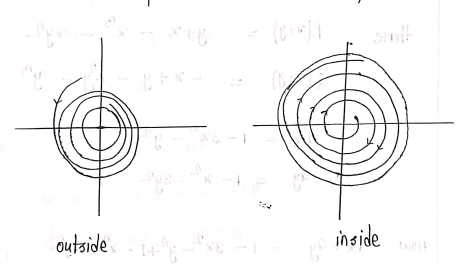
\includegraphics[]{Image/phase portrait 1.png}
\end{center}